% Schematic cross-section of a Foldscope, after Fig. 1C of
% Cybulski, Clements & Prakash, PLOS ONE 9(6): e98781 (2014).
% Not to scale. Vertical dimensions exaggerated for clarity.
\documentclass[tikz,border=4pt]{standalone}
\usetikzlibrary{arrows.meta,decorations.pathreplacing,calc}
\begin{document}
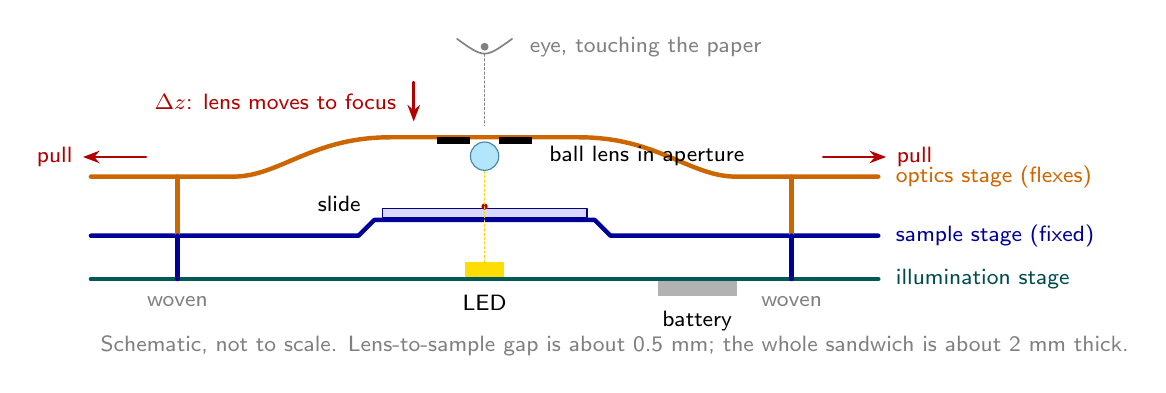
\begin{tikzpicture}[x=1cm,y=1cm,line cap=round,line join=round,
  stage/.style={line width=1.6pt},
  optics/.style={stage,draw=orange!80!black},
  sample/.style={stage,draw=blue!60!black},
  illum/.style={stage,draw=teal!70!black},
  arrow/.style={-{Stealth[length=6pt]},line width=1pt,draw=red!70!black},
  lbl/.style={font=\footnotesize\sffamily}]

% --- illumination stage (bottom): flat strip with LED and battery ----------
\draw[illum] (-5,0) -- (5,0);
\fill[yellow!80!orange] (-0.25,0.02) rectangle (0.25,0.22);   % LED
\node[lbl,anchor=north] at (0,-0.08) {LED};
\fill[gray!60] (2.2,-0.22) rectangle (3.2,-0.02);               % button cell
\node[lbl,anchor=north] at (2.7,-0.28) {battery};
\node[lbl,anchor=west,text=teal!60!black] at (5.1,0) {illumination stage};

% --- sample stage (middle): holds the slide ---------------------------------
\draw[sample] (-5,0.55) -- (-1.6,0.55) -- (-1.4,0.75) -- (1.4,0.75) -- (1.6,0.55) -- (5,0.55);
\fill[blue!15] (-1.3,0.78) rectangle (1.3,0.90);                 % glass slide
\draw[blue!50!black,line width=0.4pt] (-1.3,0.78) rectangle (1.3,0.90);
\fill[red!70!black] (0,0.92) circle (0.04);                      % specimen
\node[lbl,anchor=west,text=blue!60!black] at (5.1,0.55) {sample stage (fixed)};
\node[lbl,anchor=east] at (-1.45,0.95) {slide};

% --- optics stage (top): flexes; carries the ball lens ----------------------
% drawn as a shallow arch so the flexure reads; the lens hangs under the apex
\draw[optics] (-5,1.3) -- (-3.2,1.3)
   .. controls (-2.6,1.3) and (-2.2,1.8) .. (-1.2,1.8)
   -- (1.2,1.8)
   .. controls (2.2,1.8) and (2.6,1.3) .. (3.2,1.3)
   -- (5,1.3);
% aperture plate and ball lens
\fill[black] (-0.6,1.72) rectangle (-0.18,1.8);
\fill[black] (0.18,1.72) rectangle (0.6,1.8);
\fill[cyan!30] (0,1.56) circle (0.18);
\draw[cyan!60!black] (0,1.56) circle (0.18);
\node[lbl,anchor=west] at (0.7,1.56) {ball lens in aperture};
\node[lbl,anchor=west,text=orange!80!black] at (5.1,1.3) {optics stage (flexes)};

% --- weaving: the three stages pass through slots in each other -------------
\foreach \x in {-3.9,3.9}{
  \draw[optics] (\x,1.3) -- (\x,0.55);
  \draw[sample] (\x,0.55) -- (\x,0);
}
\node[lbl,anchor=north,gray] at (-3.9,-0.1) {woven};
\node[lbl,anchor=north,gray] at (3.9,-0.1) {woven};

% --- actions ----------------------------------------------------------------
\draw[arrow] (-4.3,1.55) -- (-5.1,1.55) node[lbl,anchor=east,text=red!70!black] {pull};
\draw[arrow] (4.3,1.55) -- (5.1,1.55) node[lbl,anchor=west,text=red!70!black] {pull};
\draw[arrow] (-0.9,2.5) -- (-0.9,2.0);
\node[lbl,anchor=east,text=red!70!black] at (-1.0,2.25) {$\Delta z$: lens moves to focus};

% light path
\draw[yellow!70!orange,line width=0.6pt,densely dotted] (0,0.22) -- (0,1.38);

% eye
\node[lbl,anchor=west,gray] at (0.45,2.95) {eye, touching the paper};
\draw[gray,line width=0.6pt] (-0.35,3.05) .. controls (0,2.8) .. (0.35,3.05);
\fill[gray] (0,2.95) circle (0.05);
\draw[gray,densely dotted,line width=0.6pt] (0,2.85) -- (0,1.95);

% scale note
\node[lbl,gray,anchor=north west] at (-5,-0.6) {Schematic, not to scale. Lens-to-sample gap is about 0.5 mm; the whole sandwich is about 2 mm thick.};
\end{tikzpicture}
\end{document}
